\documentclass[]{standalone}

\usepackage{adjustbox}

\usepackage{amsmath}

\usepackage{mathrsfs}

\usepackage{circuitikz}
\usepackage{tikz}
\usetikzlibrary{arrows, patterns, decorations.pathmorphing, backgrounds, positioning, fit, petri, shapes, trees, matrix, chains, decorations, decorations.pathreplacing, decorations.fractals, calc,snakes,trees, decorations.markings}

\usepackage{color}
\definecolor{soton}{RGB}{7,51,71}
\colorlet{comms}{red!50!yellow}
\colorlet{payld}{pink!50!purple}
\colorlet{obdh}{green!50!black}

\begin{document}

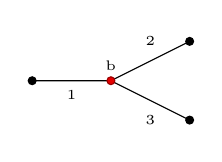
\begin{tikzpicture}

\draw (0,0) -- (1,0) -- (2,0.5);
\draw (1,0) -- (2,-0.5);
\draw[fill=black] (0,0) circle (0.05);
\draw[red!60!black, fill=red!90!black] (1,0) node[above, black] {\tiny{b}} circle (0.05);
\draw[fill=black] (2,0.5) circle (0.05);
\draw[fill=black] (2,-0.5) circle (0.05);
\node[below] at (0.5,0) {\tiny{1}};
\node[] at (1.5,0.5) {\tiny{2}};
\node[] at (1.5,-0.5) {\tiny{3}};

\end{tikzpicture}


\end{document}